\documentclass[12pt, a4paper]{article}
\usepackage[utf8]{inputenc}
\usepackage[T1]{fontenc}
\usepackage[slovak]{babel}
\usepackage{geometry}
\geometry{margin=2.5cm}
\usepackage{graphicx}
\usepackage{hyperref}
\hypersetup{colorlinks=true, linkcolor=black, urlcolor=blue}
\usepackage{parskip}
\usepackage{titlesec}
\usepackage{listings}
\usepackage{xcolor}
\usepackage{float}
\usepackage{microtype}

\lstset{
  basicstyle=\ttfamily\small,
  breaklines=true,
  frame=none,
  backgroundcolor=\color{gray!8},
  xleftmargin=4pt,
  xrightmargin=4pt,
}

\titleformat{\section}{\large\bfseries}{}{0em}{}
\titleformat{\subsection}{\normalsize\bfseries\color{black!70}}{}{0em}{}

\begin{document}

% ── Titulná strana ──────────────────────────────────────────────────────────
\begin{titlepage}
  \centering
  \vspace*{1cm}
  {\large Slovenská Technická Univerzita, Bratislava\\}
  {\large Fakulta Informatiky a Informačných Technológií\\}
  \vfill
  {\LARGE\bfseries Elektronický obchod -- semestrálny projekt\\}
  \vspace{0.5em}
  {\large Základy webových technológií\\}
  \vfill
  \begin{flushleft}
    10.~5.~2025 \hfill Jakub Kelemen\\
    Bratislava    \hfill Martin Stavrovsky
  \end{flushleft}
\end{titlepage}

% ── Obsah ───────────────────────────────────────────────────────────────────
\tableofcontents
\newpage

% ── Zadanie ─────────────────────────────────────────────────────────────────
\section{Zadanie}

Našou úlohou bolo vytvoriť vlastnú webovú aplikáciu~-- e‑shop zameraný na predaj prémiových kávových zŕn. Aplikácia komplexne rieši typické prípady použitia elektronického obchodu a~pozostáva z~klientskej aj administrátorskej časti.

V~rámci klientskej časti sme implementovali funkcie ako prehľad produktov s~filtrovaním a~stránkovaním, detail produktu, nákupný košík, registráciu, prihlásenie, možnosť uskutočniť objednávku a~ukladanie obľúbených produktov. Administrátorská časť obsahuje správu produktov (vytváranie, úprava, mazanie vrátane nahrávanie obrázkov).

Projekt bol vypracovávaný v~dvoch hlavných fázach. V~prvej fáze sme tvorili návrh používateľského rozhrania v~podobe skíc a~návrh dátového modelu. Z~týchto skíc sme následne vytvorili HTML a~CSS šablóny, ktoré sú plne responzívne. V~druhej fáze projektu sme aplikovali PHP framework Laravel, ktorý využíva server-side rendering. Vďaka tomu sa nám podarilo vytvoriť plne funkčný interaktívny e‑shop.

% ── Databáza ────────────────────────────────────────────────────────────────
\section{Databáza}

Pracujeme s~databázovým systémom \textbf{PostgreSQL}. Databáza obsahuje deväť hlavných tabuliek, ktoré spoločne pokrývajú všetky požadované prípady použitia.

\subsection{Fyzický dátový model}

Fyzický model databázy je znázornený na obrázku~\ref{fig:fyzicky_model}. Tabuľky a~ich vzťahy:

\begin{itemize}
  \item \textbf{users} -- zákazníci a~administrátori; rozlíšenie roľou \texttt{role} (\texttt{customer}/\texttt{admin}).
  \item \textbf{categories} -- kategórie kávy (napr.\ Single Origin, Blend, Decaf); atribúty \texttt{name} a~\texttt{slug}.
  \item \textbf{products} -- hlavná tabuľka produktov; cudzí kľúč na \texttt{categories}; atribúty \texttt{name}, \texttt{slug}, \texttt{description}, \texttt{price}, \texttt{stock\_quantity}, \texttt{is\_active}, \texttt{origin\_label}, \texttt{roast\_level}, \texttt{weight\_grams}.
  \item \textbf{product\_images} -- obrázky produktov; cudzí kľúč na \texttt{products}; atribút \texttt{path} (relatívna cesta k~súboru), \texttt{sort\_order}.
  \item \textbf{cart\_items} -- položky nákupného košíka; cudzí kľúč na \texttt{users} (nullable pre hostí) a~na \texttt{products}; atribúty \texttt{session\_id} (pre hostí), \texttt{quantity}.
  \item \textbf{favorites} -- obľúbené produkty; cudzí kľúč na \texttt{users} a~\texttt{products}; unikátna kombinácia \texttt{(user\_id, product\_id)}.
  \item \textbf{addresses} -- uložené doručovacie adresy používateľa; cudzí kľúč na \texttt{users}; atribúty \texttt{first\_name}, \texttt{last\_name}, \texttt{email}, \texttt{address\_line}, \texttt{city}, \texttt{state}, \texttt{postal\_code}, \texttt{is\_default}.
  \item \textbf{orders} -- história objednávok; cudzí kľúč na \texttt{users} (nullable -- hosťovský checkout); snapshot doručovacích údajov, \texttt{shipping\_method}, \texttt{shipping\_price}, \texttt{subtotal}, \texttt{tax}, \texttt{total}, \texttt{status}.
  \item \textbf{order\_items} -- položky objednávky; cudzí kľúč na \texttt{orders} (cascade) a~\texttt{products} (nullable); snapshot \texttt{product\_name} a~\texttt{unit\_price} v~čase objednávky, \texttt{quantity}, \texttt{line\_total}.
\end{itemize}

\begin{figure}[H]
  \centering
  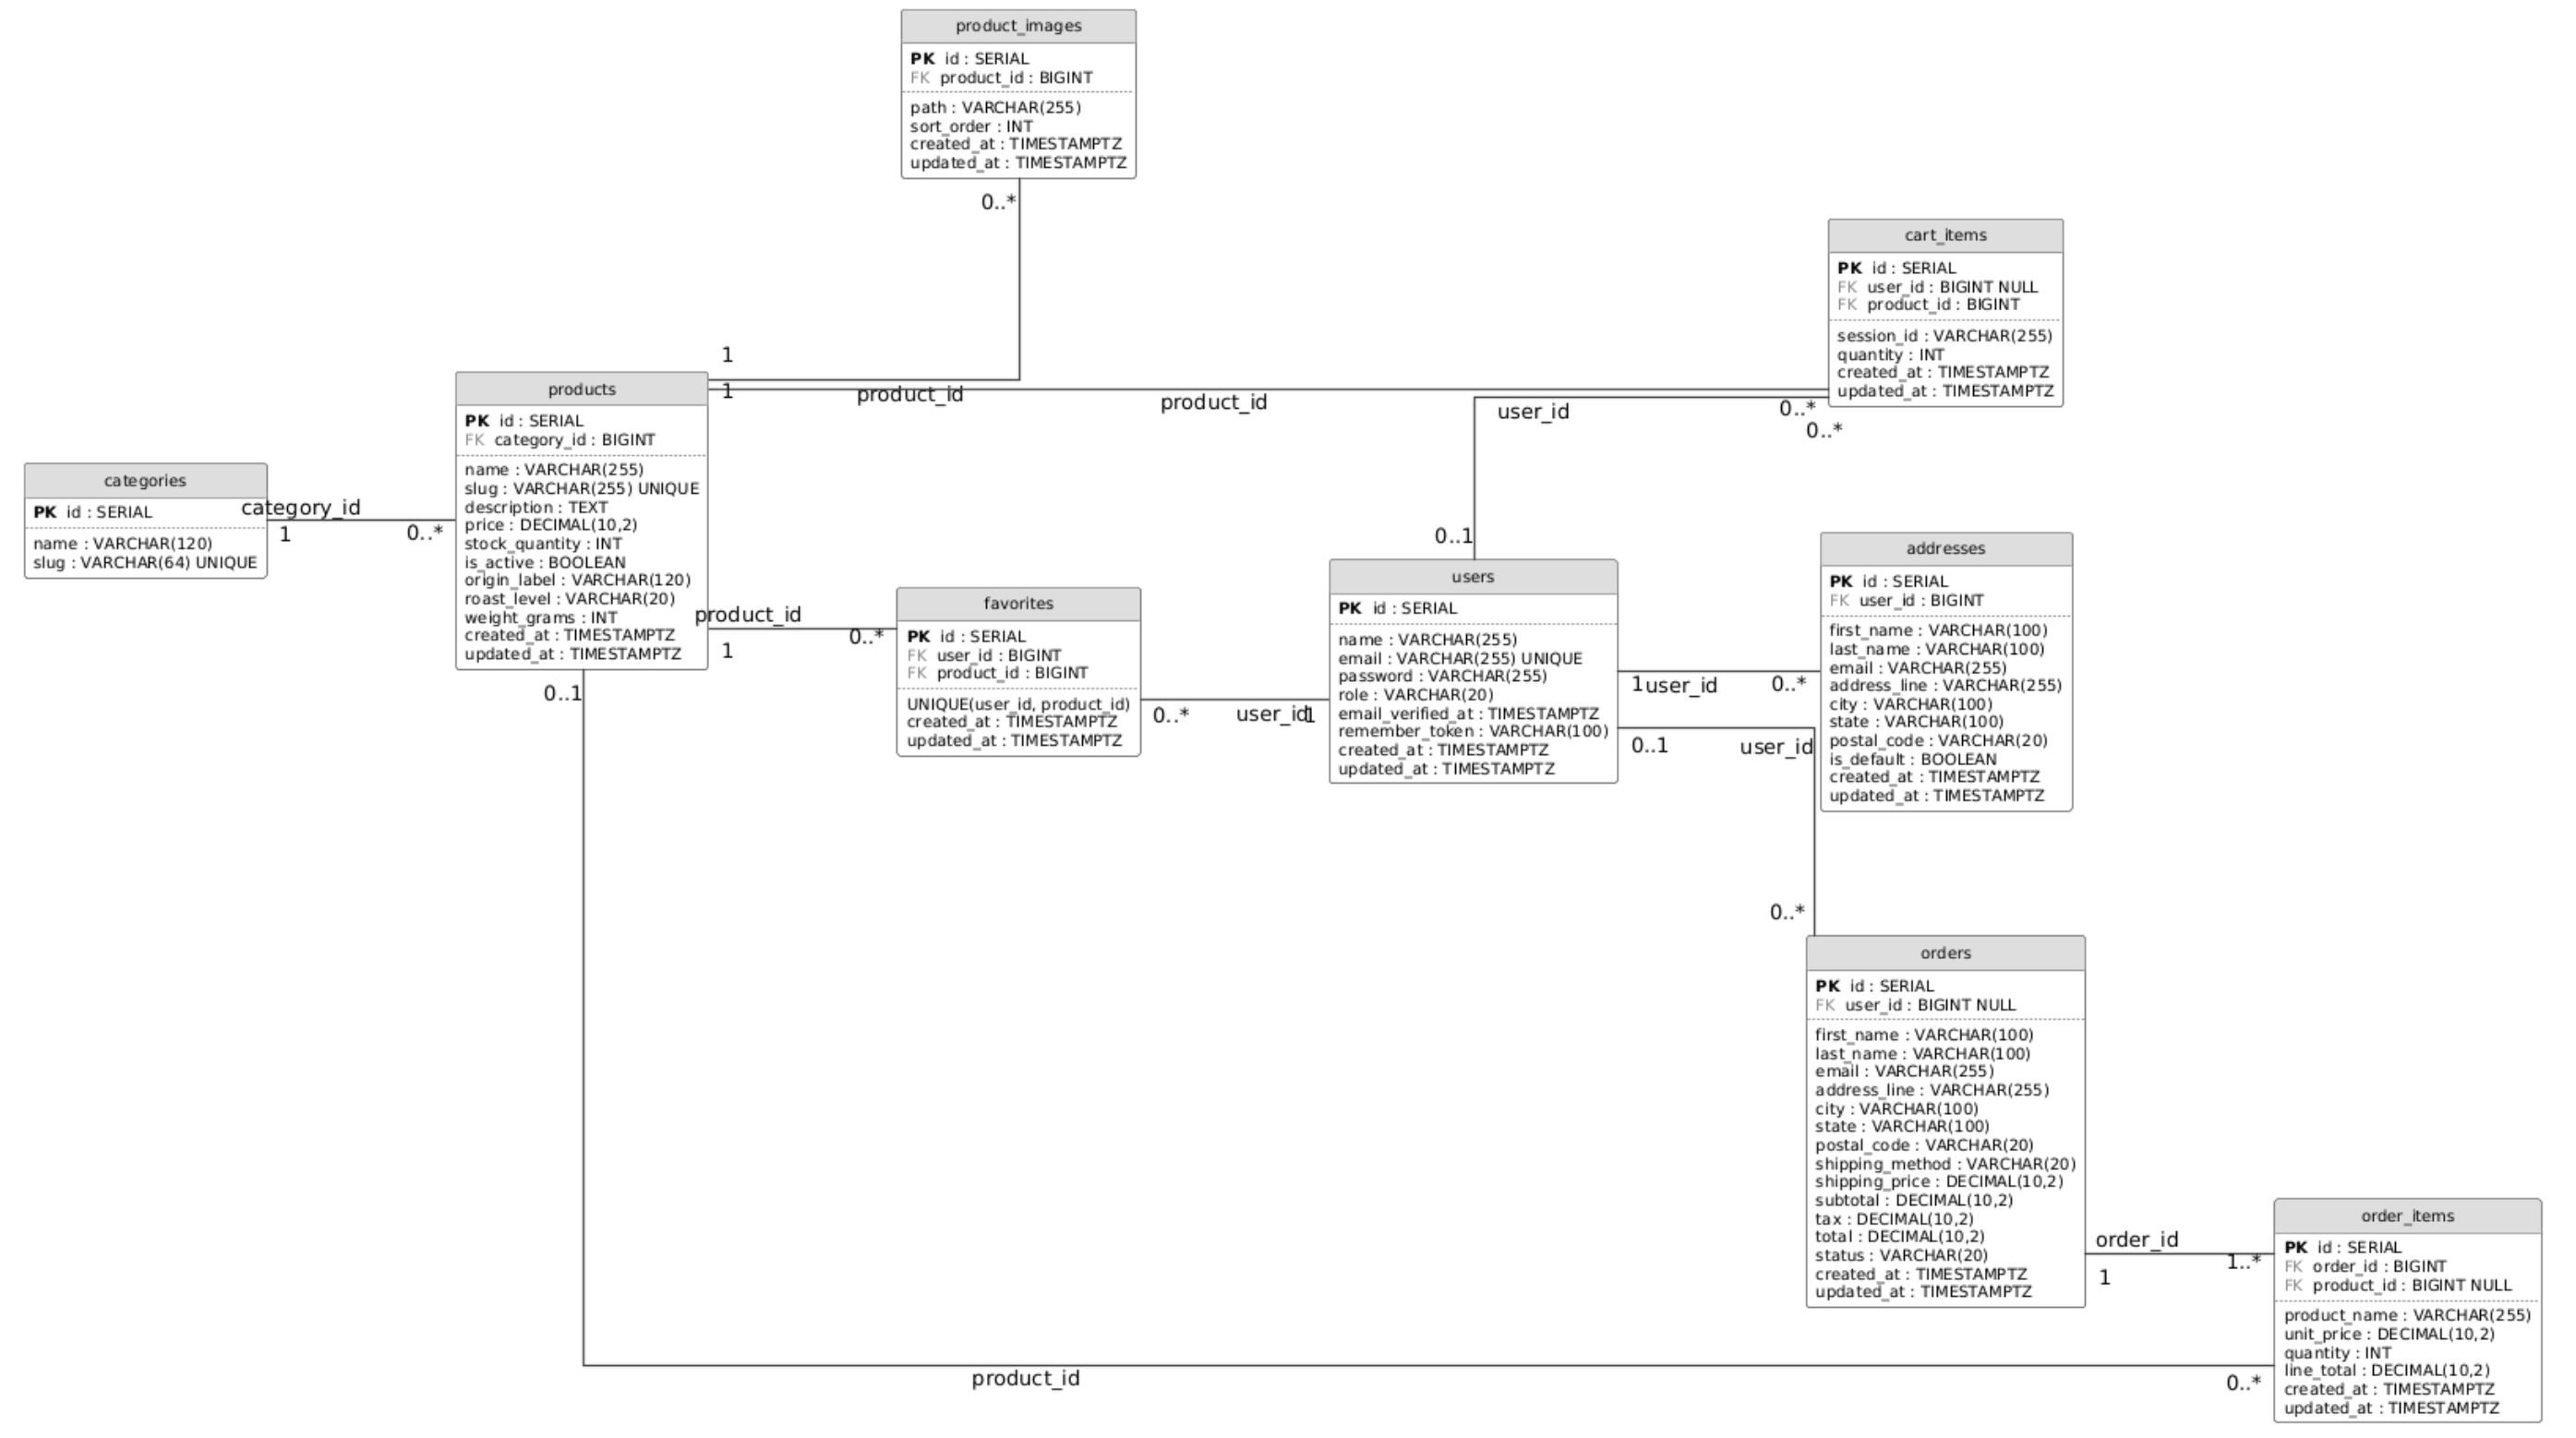
\includegraphics[width=\linewidth, height=0.85\textheight, keepaspectratio]{figures/fyzicky_model.png}
  \caption{Fyzický dátový model databázy}
  \label{fig:fyzicky_model}
\end{figure}

\subsection{Zmeny v~dátovom modeli oproti fáze~1}

Pôvodný fyzický model z~fázy~1 obsahoval tabuľky \texttt{category}, \texttt{category\_product}, \texttt{product}, \texttt{user}, \texttt{address}, \texttt{order} a~\texttt{order\_item}. V~implementácii sme vykonali nasledovné zmeny:

\textbf{Odstránená junction tabuľka \texttt{category\_product}.}
Pôvodný návrh počítal so vzťahom M:N medzi produktom a~kategóriou (jeden produkt mohol patriť do viacerých kategórií). Rozhodli sme sa zjednodušiť model na vzťah 1:N -- každý produkt patrí práve do jednej kategórie. Atribút \texttt{category\_id} je preto priamo cudzím kľúčom v~tabuľke \texttt{products}, junction tabuľka nie je potrebná.

\textbf{Rozšírená tabuľka \texttt{products}.}
Oproti pôvodnému návrhu sme pridali atribúty špecifické pre kávu: \texttt{roast\_level} (stupeň praženia: light/medium/dark), \texttt{weight\_grams} (hmotnosť balenia v~gramoch) a~\texttt{slug} (URL-priateľský identifikátor). Atribút \texttt{origin\_label} bol v~pôvodnom modeli plánovaný a~zostal zachovaný. Tieto atribúty umožňujú bohatšie filtrovanie.

\textbf{Nová tabuľka \texttt{product\_images}.}
Pôvodný model nepočítal s~viacerými obrázkami na produkt. Vytvorili sme samostatnú tabuľku s~atribútmi \texttt{path} (relatívna cesta k~súboru na disku) a~\texttt{sort\_order} (poradie zobrazenia). Jeden produkt môže mať ľubovoľný počet obrázkov.

\textbf{Nová tabuľka \texttt{cart\_items}.}
Pôvodný model neobsahoval tabuľku košíka -- predpokladalo sa, že košík bude riešený výlučne cez session. Pridali sme tabuľku \texttt{cart\_items} s~cudzím kľúčom \texttt{user\_id} (nullable) a~\texttt{session\_id} pre hostí. Toto riešenie umožňuje perzistenciu košíka pre prihlásených používateľov a~zároveň hosťovský checkout bez registrácie.

\textbf{Nová tabuľka \texttt{favorites}.}
Tabuľka nebola v~pôvodnom návrhu. Obsahuje cudzí kľúč \texttt{user\_id} a~\texttt{product\_id} s~unikátnou kombináciou, čo zabraňuje duplicitným zápisom. Slúži na ukladanie obľúbených produktov zákazníka a~ich zobrazenie v~profile.

\textbf{Zmenená tabuľka \texttt{users}.}
Pôvodný atribút \texttt{password\_hash} bol premenovaný na \texttt{password} (Laravel bcrypt hash). Pridané atribúty: \texttt{name} (celé meno), \texttt{remember\_token} (pre funkciu „zapamätaj ma") a~\texttt{email\_verified\_at}. Atribút \texttt{last\_login\_at} bol odstránený ako nepotrebný. Rola je uložená ako reťazec \texttt{role} (\texttt{customer}/\texttt{admin}) namiesto ENUM.

\textbf{Implementované tabuľky \texttt{addresses}, \texttt{orders} a~\texttt{order\_items}.}
Oproti pôvodnému záznamu z~fázy~1 sme všetky tri tabuľky zachovali a~naplno implementovali. Prihlásený používateľ si môže počas checkoutu uložiť doručovaciu adresu do tabuľky \texttt{addresses} (zaškrtávacie pole ``Save this address''). Pri ďalšej objednávke sa formulár predvyplní uloženou predvolenou adresou. Po dokončení checkoutu sa vytvorí záznam v~tabuľke \texttt{orders} so snapshotom doručovacích a~cenových údajov a~záznamy v~\texttt{order\_items} so snapshotom názvu a~ceny každého produktu -- história objednávok tým zostáva konzistentná aj po budúcich zmenách cien alebo produktov. História objednávok je dostupná v~profile používateľa.

% ── Návrhové rozhodnutia ────────────────────────────────────────────────────
\section{Návrhové rozhodnutia}

\textbf{PHP framework Laravel} sme si zvolili, pretože je odporúčaný v~rámci predmetu a~poskytuje robustnú základnú sadu nástrojov: ORM (Eloquent), systém migrácie databázy, Blade šablóny a~vstavaný autentifikačný systém. Vďaka Laravelu sme zvládli vytvoriť backendovú logiku bez potreby prídavných knižníc.

\textbf{PostgreSQL} sme zvolili ako databázový systém, pretože máme s~ním skúsenosti z~predmetu Databázové systémy a~dokázal pokryť všetky naše požiadavky vrátane cizích kľúčov, kaskádového mazania a~unikátnych obmedzení.

\textbf{Bootstrap 5} sme využili pre používateľské rozhranie, pretože poskytuje preddefinované komponenty, responzívny grid systém a~konzistentný vizuálny štýl. Bootstrap je do projektu zahrnutý cez CDN v~\texttt{layouts/app.blade.php}.

\textbf{Obrázky produktov} sa fyzicky ukladajú do \texttt{storage/app/public/products/} pomocou Laravel \texttt{Storage} facade. V~databáze je uložená iba relatívna cesta k~súboru (napr.\ \texttt{storage/products/abc.jpg}), nie binárny obsah. Prístup k~obrázkom je zabezpečený symbolickým odkazom \texttt{public/storage} vytvoreným príkazom \texttt{php artisan storage:link}.

\textbf{Perzistencia košíka} je riešená dvojako: pre prihlásených používateľov sú položky uložené v~databáze v~tabuľke \texttt{cart\_items} s~väzbou na \texttt{user\_id}; pre hostí sa využíva Laravel session s~\texttt{session\_id}. Pri prihlásení sa hosťovský košík automaticky zlúči s~databázovým košíkom prihláseného používateľa pomocou triedy \texttt{GuestCartMerger}.

\textbf{Systém rolí} je implementovaný jednoduchým atribútom \texttt{role} v~tabuľke \texttt{users} s~hodnotami \texttt{customer} a~\texttt{admin}. Prístup do administrátorského rozhrania je chránený middleware \texttt{EnsureUserIsAdmin}, ktorý overuje rolu a~vracia HTTP~403 pri neoprávnenom prístupe.

\textbf{Validácia formulárov} prebieha na dvoch úrovniach. Na strane klienta JavaScript okamžite obmedzuje vstup (napr.\ číslo karty -- len číslice, max.\ 16~znakov; CVV~-- presne 3~číslice; formát expirácie MM/YY vrátane kontroly, že dátum nie je v~minulosti; PSČ -- len číslice). Na strane servera Laravel \texttt{Request::validate()} overuje všetky dáta pred spracovaním vrátane rovnakej kontroly expirácie pomocou closure pravidla -- tento prístup zabezpečuje integritu aj pri vypnutom JavaScripte.

% ── Opis implementácie ──────────────────────────────────────────────────────
\section{Opis implementácie vybraných prípadov použitia}

\subsection{Prihlásenie}

Prihlásenie spracováva \texttt{AuthController} v~metóde \texttt{login()}. Používateľ vyplní formulár v~\texttt{src/auth/login.blade.php} s~poliami \texttt{email} a~\texttt{password} a~odošle ho POST požiadavkou na rovnakú URL.

Server najprv validuje vstupy (\texttt{required}, \texttt{email}), následne volá \texttt{Auth::attempt()} s~prihlasovacími údajmi. Ak Laravel nájde zhodu v~tabuľke \texttt{users} a~heslo zodpovedá bcrypt hashu, session sa regeneruje (\texttt{regenerate()}) a~hosťovský košík sa zlúči s~databázovým. Používateľ je presmerovaný na domovskú stránku.

Pri nesprávnych údajoch vráti \texttt{Auth::attempt()} \texttt{false}, server volá \texttt{back()->withErrors()} a~chybová hláška sa zobrazí v~šablóne pomocou direktívy \texttt{@error}.

Registrácia prebieha analogicky -- \texttt{register()} validuje unikátnosť emailu, heslo (min. 8 znakov, potvrdenie), vytvorí záznam cez \texttt{User::create()} s~hashovaným heslom a~ihneď prihlási nového používateľa cez \texttt{Auth::login()}.

\subsection{Vyhľadávanie}

Full-text vyhľadávanie je implementované v~\texttt{ShopController::index()}. Formulár odosiela GET požiadavku s~parametrom \texttt{q} na URL \texttt{/src/public/shop.php}.

Ak je parameter \texttt{q} neprázdny, controller zostaví SQL LIKE podmienku a~aplikuje ju na query pomocou Eloquent:

\begin{lstlisting}
$like = '%' . Str::lower($search) . '%';
$query->where(function ($q) use ($like) {
    $q->whereRaw('LOWER(name) LIKE ?', [$like])
      ->orWhereRaw('LOWER(description) LIKE ?', [$like])
      ->orWhereRaw('LOWER(COALESCE(origin_label, '')) LIKE ?', [$like])
      ->orWhereRaw('LOWER(roast_level) LIKE ?', [$like])
      ->orWhereHas('category', function ($cq) use ($like) {
          $cq->whereRaw('LOWER(name) LIKE ?', [$like]);
      });
});
\end{lstlisting}

Vyhľadávanie je teda case-insensitive a~pokrýva názov produktu, popis, krajinu pôvodu, stupeň praženia aj názov kategórie. Výsledky prechádzajú rovnakým stránkovaním a~filtrovaním ako bežný výpis.

\subsection{Pridanie produktu do košíka}

Používateľ môže pridať produkt do košíka z~výpisu produktov alebo z~detailu. Formulár odosiela POST požiadavku na \texttt{/cart/add} so skrytými poliami \texttt{product\_id} a~\texttt{quantity}.

Spracovanie prebieha v~\texttt{CartController::add()}:

\begin{itemize}
  \item \textbf{Prihlásený používateľ:} controller hľadá existujúci záznam v~\texttt{cart\_items} podľa \texttt{user\_id} a~\texttt{product\_id}. Ak existuje, zvýši \texttt{quantity}; ak nie, vytvorí nový záznam.
  \item \textbf{Hosť:} košík je uložený v~Laravel session. Controller načíta pole \texttt{session('cart')}, upraví množstvo alebo pridá novú položku a~session aktualizuje.
\end{itemize}

Controller tiež overuje dostupnosť na sklade (\texttt{stock\_quantity}) a~zamietne pridanie, ak by požadované množstvo prekročilo zásoby.

\subsection{Stránkovanie}

Stránkovanie je implementované v~\texttt{ShopController::index()} pomocou Eloquent metódy \texttt{paginate(6)}, ktorá automaticky číta parameter \texttt{page} z~URL a~vracia \texttt{LengthAwarePaginator}.

\begin{lstlisting}
$products = $query->paginate($perPage)->withQueryString();
\end{lstlisting}

Volanie \texttt{withQueryString()} zabezpečí, že všetky aktuálne filtre a~vyhľadávací reťazec sa zachovajú v~URL pri prechode na inú stránku. V~Blade šablóne sa stránkovanie vykreslí pomocou:

\begin{lstlisting}
{{ $products->withQueryString()->links('vendor.pagination.bootstrap-5') }}
\end{lstlisting}

Laravelovský paginator generuje HTML s~Bootstrap 5 triedami, takže stránkovanie je vizuálne konzistentné so zvyškom aplikácie.

\subsection{Základné filtrovanie}

Filtrovanie produktov je implementované v~\texttt{ShopController::index()} a~podporuje štyri atribúty: kategóriu, stupeň praženia (roast level), krajinu pôvodu a~cenové rozpätie.

Každý filter číta zodpovedajúci GET parameter a~podmienečne rozširuje Eloquent query:

\begin{lstlisting}
// Kategoria
if ($category !== '' && $category !== 'all') {
    $query->whereHas('category',
        fn($q) => $q->where('slug', $category));
}
// Roast level
if ($roast !== '' && $roast !== 'all') {
    $query->where('roast_level', $roast);
}
// Cenove rozpatie
if ($priceMin !== null) $query->where('price', '>=', $priceMin);
if ($priceMax !== null) $query->where('price', '<=', $priceMax);
\end{lstlisting}

Filtre sa odošlú GET formulárom, čo umožňuje záložkovateľné URL. V~šablóne sú filtre vykreslené ako tlačidlá, pričom aktívny filter je vizuálne odlíšený triedou \texttt{btn-dark}.

\subsection{Admin -- pridanie produktu}

Administrátor pristupuje k~formuláru na \texttt{/src/admin/product-add.php} (chránené middleware \texttt{auth} + \texttt{admin}). Formulár obsahuje polia: názov, kategória (select z~DB), cena, krajina pôvodu, stupeň praženia, hmotnosť, množstvo na sklade, popis a~upload obrázkov.

Po odoslaní formuláru POST požiadavkou spracováva \texttt{AdminController::store()}:

\begin{enumerate}
  \item Server validuje všetky polia pomocou \texttt{Request::validate()} -- povinné polia, číselné hodnoty, existencia kategórie v~DB, formát obrázkov (jpg/png, max 5~MB).
  \item Vygeneruje sa unikátny \texttt{slug} z~názvu produktu (kontrola duplicity v~slučke).
  \item Produkt sa uloží do tabuľky \texttt{products} cez \texttt{Product::create()}.
  \item Pre každý nahraný súbor sa zavolá \texttt{\$file->store('products', 'public')}, ktorý uloží obrázok do \texttt{storage/app/public/products/} a~vráti relatívnu cestu. Cesta sa zapíše do tabuľky \texttt{product\_images}.
  \item Administrátor je presmerovaný na dashboard so flash správou o~úspešnom vytvorení.
\end{enumerate}

\subsection{Ukladanie adresy a~história objednávok}

Na stránke doručovacích údajov (krok~1 checkoutu) je pre prihlásených používateľov zobrazené zaškrtávacie pole ``Save this address to my profile''. Ak ho zákazník zaškrtne, \texttt{CheckoutController::storeShipping()} po úspešnej validácii uloží adresu do tabuľky \texttt{addresses}. Prvá uložená adresa dostane príznak \texttt{is\_default = true}. Pri ďalšej návšteve stránky doručenia \texttt{showShipping()} predvyplní formulár predvolenou adresou používateľa z~databázy (ak v~session ešte nie sú uložené žiadne údaje).

Po prechode všetkými tromi krokmi checkoutu a~kliknutí na ``Place Order'' vykoná \texttt{completeOrder()} tieto kroky:

\begin{enumerate}
  \item Načíta položky košíka zo session alebo z~tabuľky \texttt{cart\_items}.
  \item Vypočíta poštovné a~DPH.
  \item Vytvorí záznam v~tabuľke \texttt{orders} so snapshotom doručovacích údajov a~cenových súčtov.
  \item Pre každú položku košíka vytvorí záznam v~\texttt{order\_items} so snapshotom názvu produktu, jednotkovej ceny a~celkovej sumy riadku.
  \item Vyprázdni košík a~vymaže checkout session.
\end{enumerate}

História objednávok je zobrazená v~profile používateľa -- každá objednávka ukazuje číslo objednávky, dátum, stav, doručovaciu adresu, spôsob dopravy a~tabuľku s~nakúpenými položkami.

\subsection{Admin -- odstránenie produktu}

Na admin dashboarde je pri každom produkte tlačidlo Delete. Po kliknutí sa zobrazí natívny \texttt{confirm()} dialóg s~názvom produktu. Pri potvrdení sa odošle POST formulár na \texttt{/src/admin/product-delete.php} s~\texttt{product\_id}.

Spracovanie v~\texttt{AdminController::destroy()}:

\begin{enumerate}
  \item Nájde sa produkt vrátane vzťahu \texttt{images} jedným dotazom (\texttt{with('images')}).
  \item Pre každý obrázok, ktorého cesta začína \texttt{storage/}, sa zavolá \texttt{Storage::disk('public')->delete()}, čím sa fyzický súbor vymaže z~disku.
  \item Samotný produkt sa vymaže zavolaním \texttt{\$product->delete()}; vďaka \texttt{cascadeOnDelete()} v~migrácii sa automaticky vymažú aj záznamy v~\texttt{product\_images}, \texttt{cart\_items} a~\texttt{favorites}.
  \item Administrátor je presmerovaný späť na dashboard s~potvrdením.
\end{enumerate}

% ── Snímky obrazoviek ───────────────────────────────────────────────────────
\section{Snímky obrazoviek}

\begin{figure}[H]
  \centering
  \includegraphics[width=\linewidth, height=0.85\textheight, keepaspectratio]{figures/home_page.php.png}
  \caption{Domovská stránka e-shopu s~prehľadom odporúčaných produktov.}
\end{figure}

\begin{figure}[H]
  \centering
  \includegraphics[width=\linewidth, height=0.85\textheight, keepaspectratio]{figures/produkty.png}
  \caption{Stránka výpisu produktov s~filtrovaním, zoradením a~stránkovaním.}
\end{figure}

\begin{figure}[H]
  \centering
  \includegraphics[width=\linewidth, height=0.85\textheight, keepaspectratio]{figures/detail_produktu.png}
  \caption{Detail produktu -- galéria obrázkov, specs, výber množstva, pridanie do košíka a~obľúbené.}
\end{figure}

\begin{figure}[H]
  \centering
  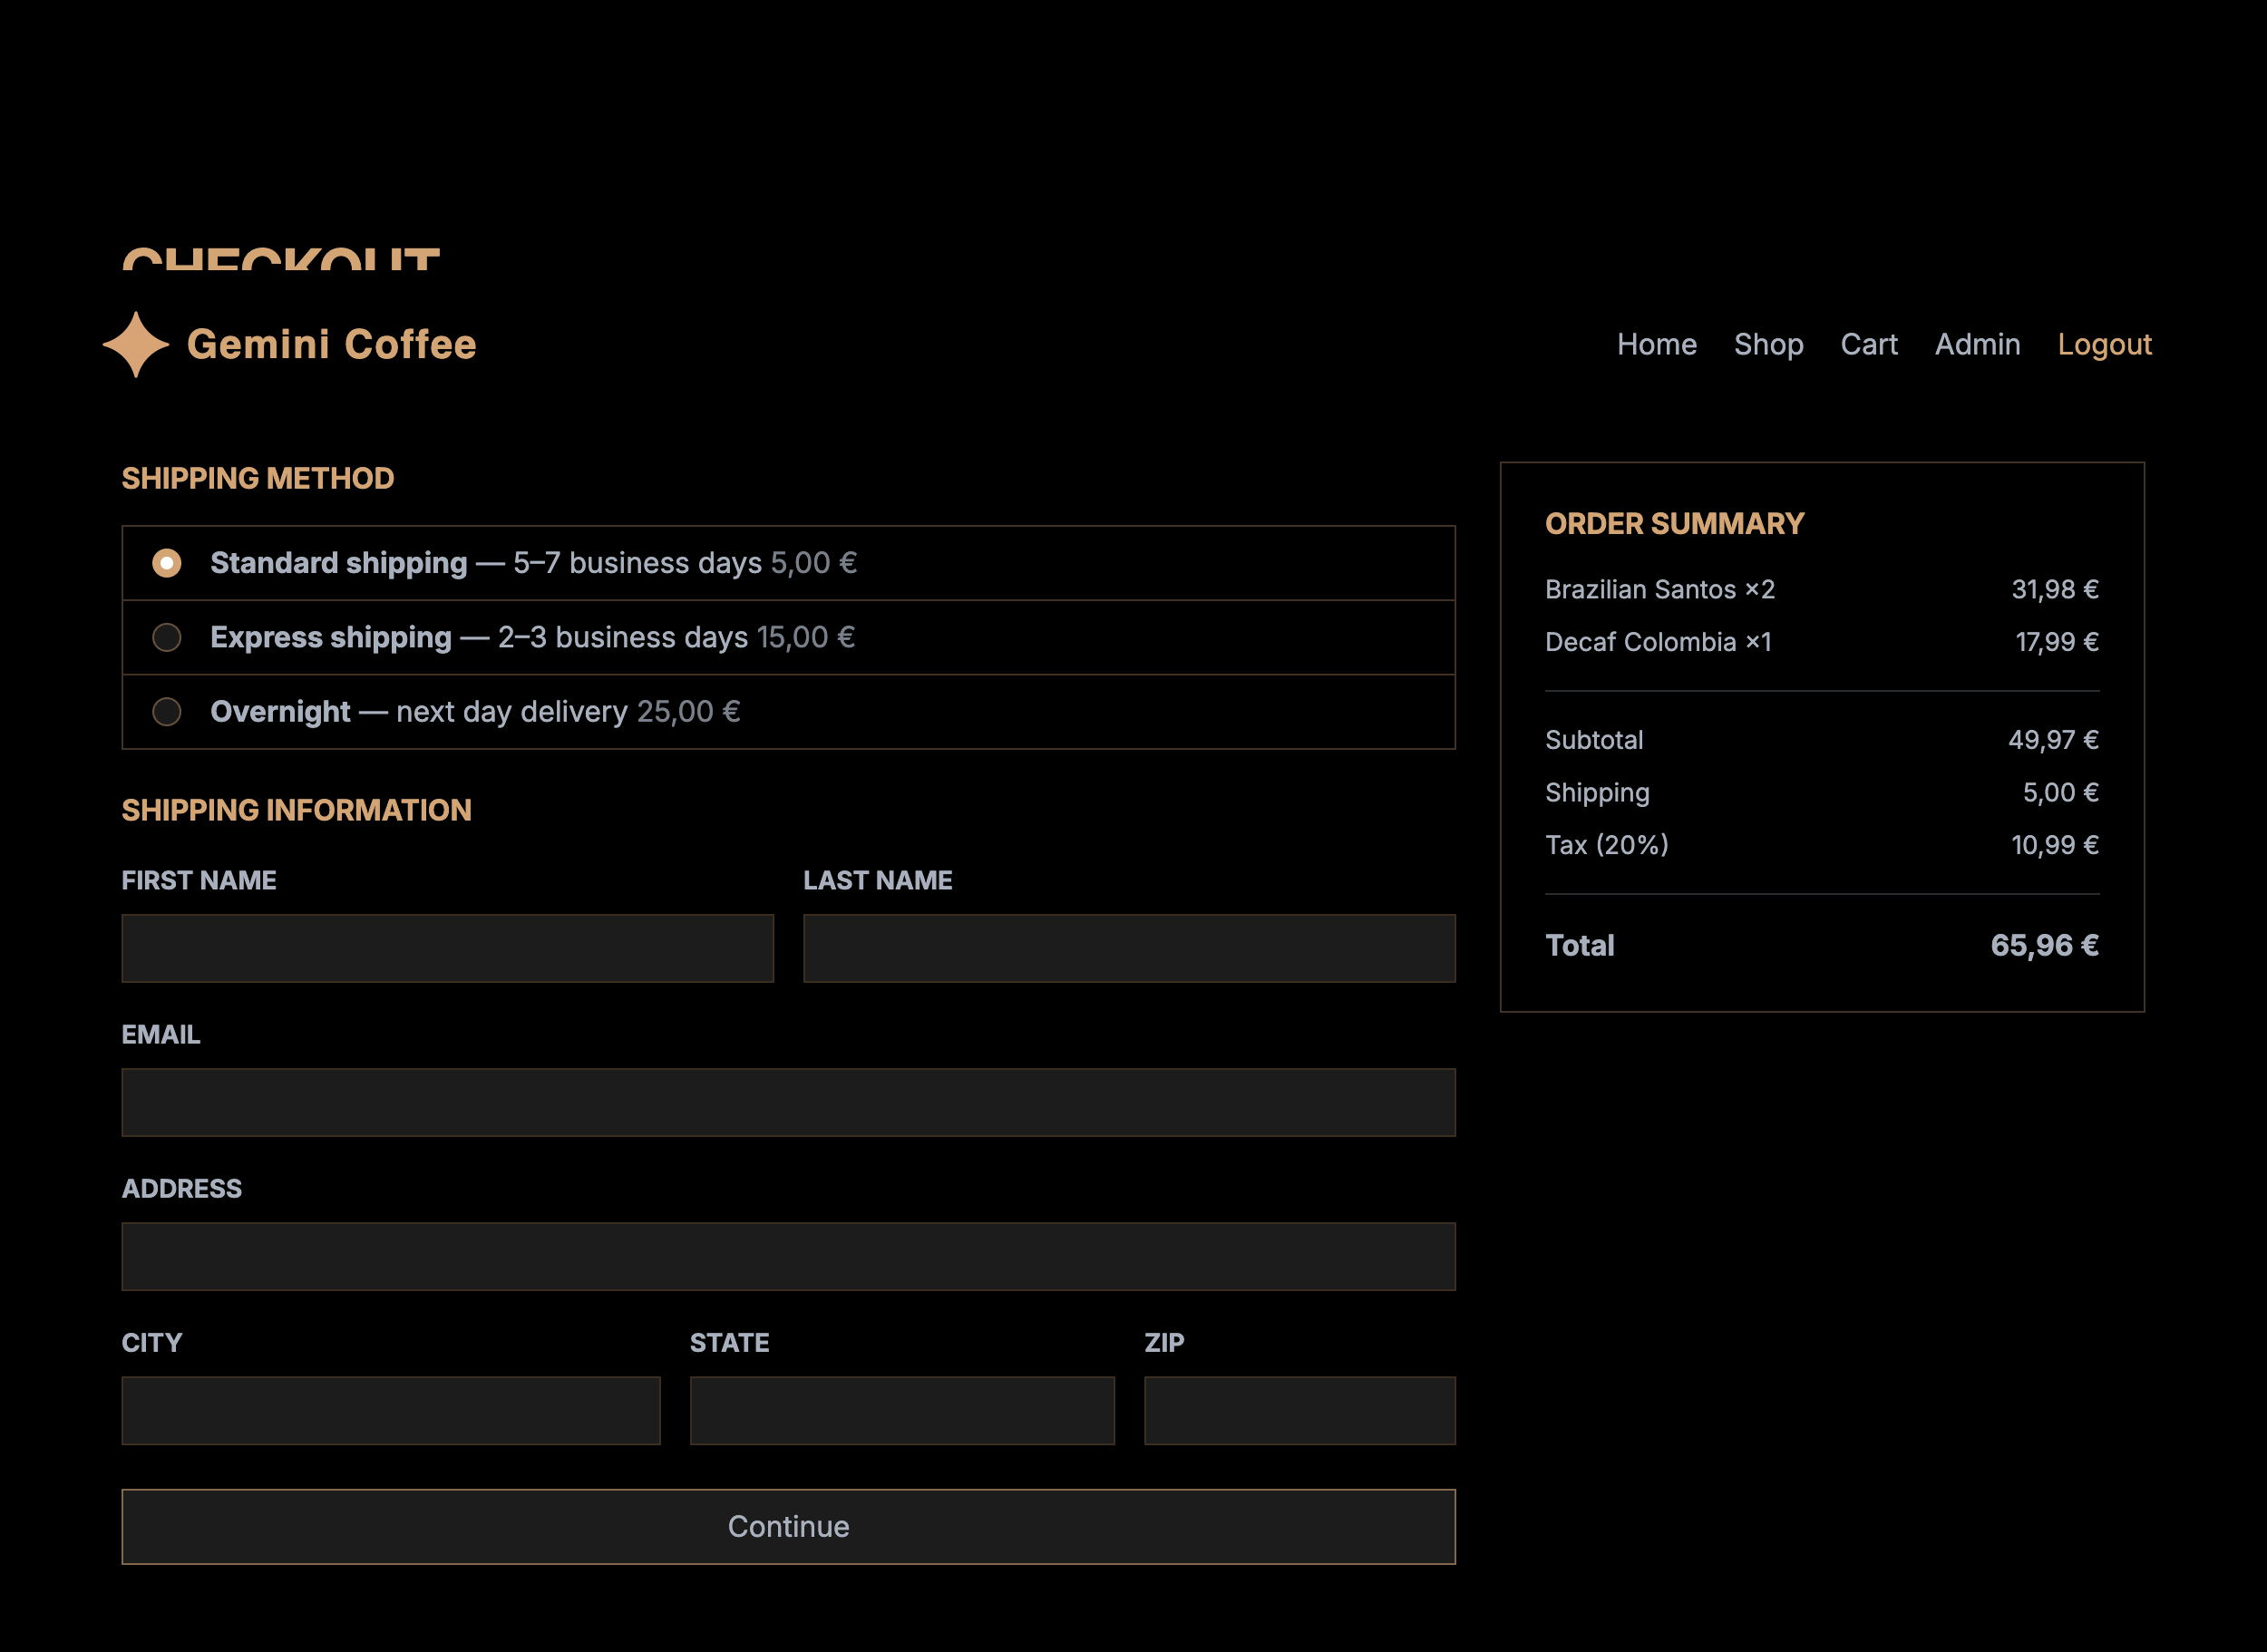
\includegraphics[width=\linewidth, height=0.85\textheight, keepaspectratio]{figures/cart1.png}
  \caption{Nákupný košík s~možnosťou zmeny množstva a~odstránenia položiek.}
\end{figure}

\begin{figure}[H]
  \centering
  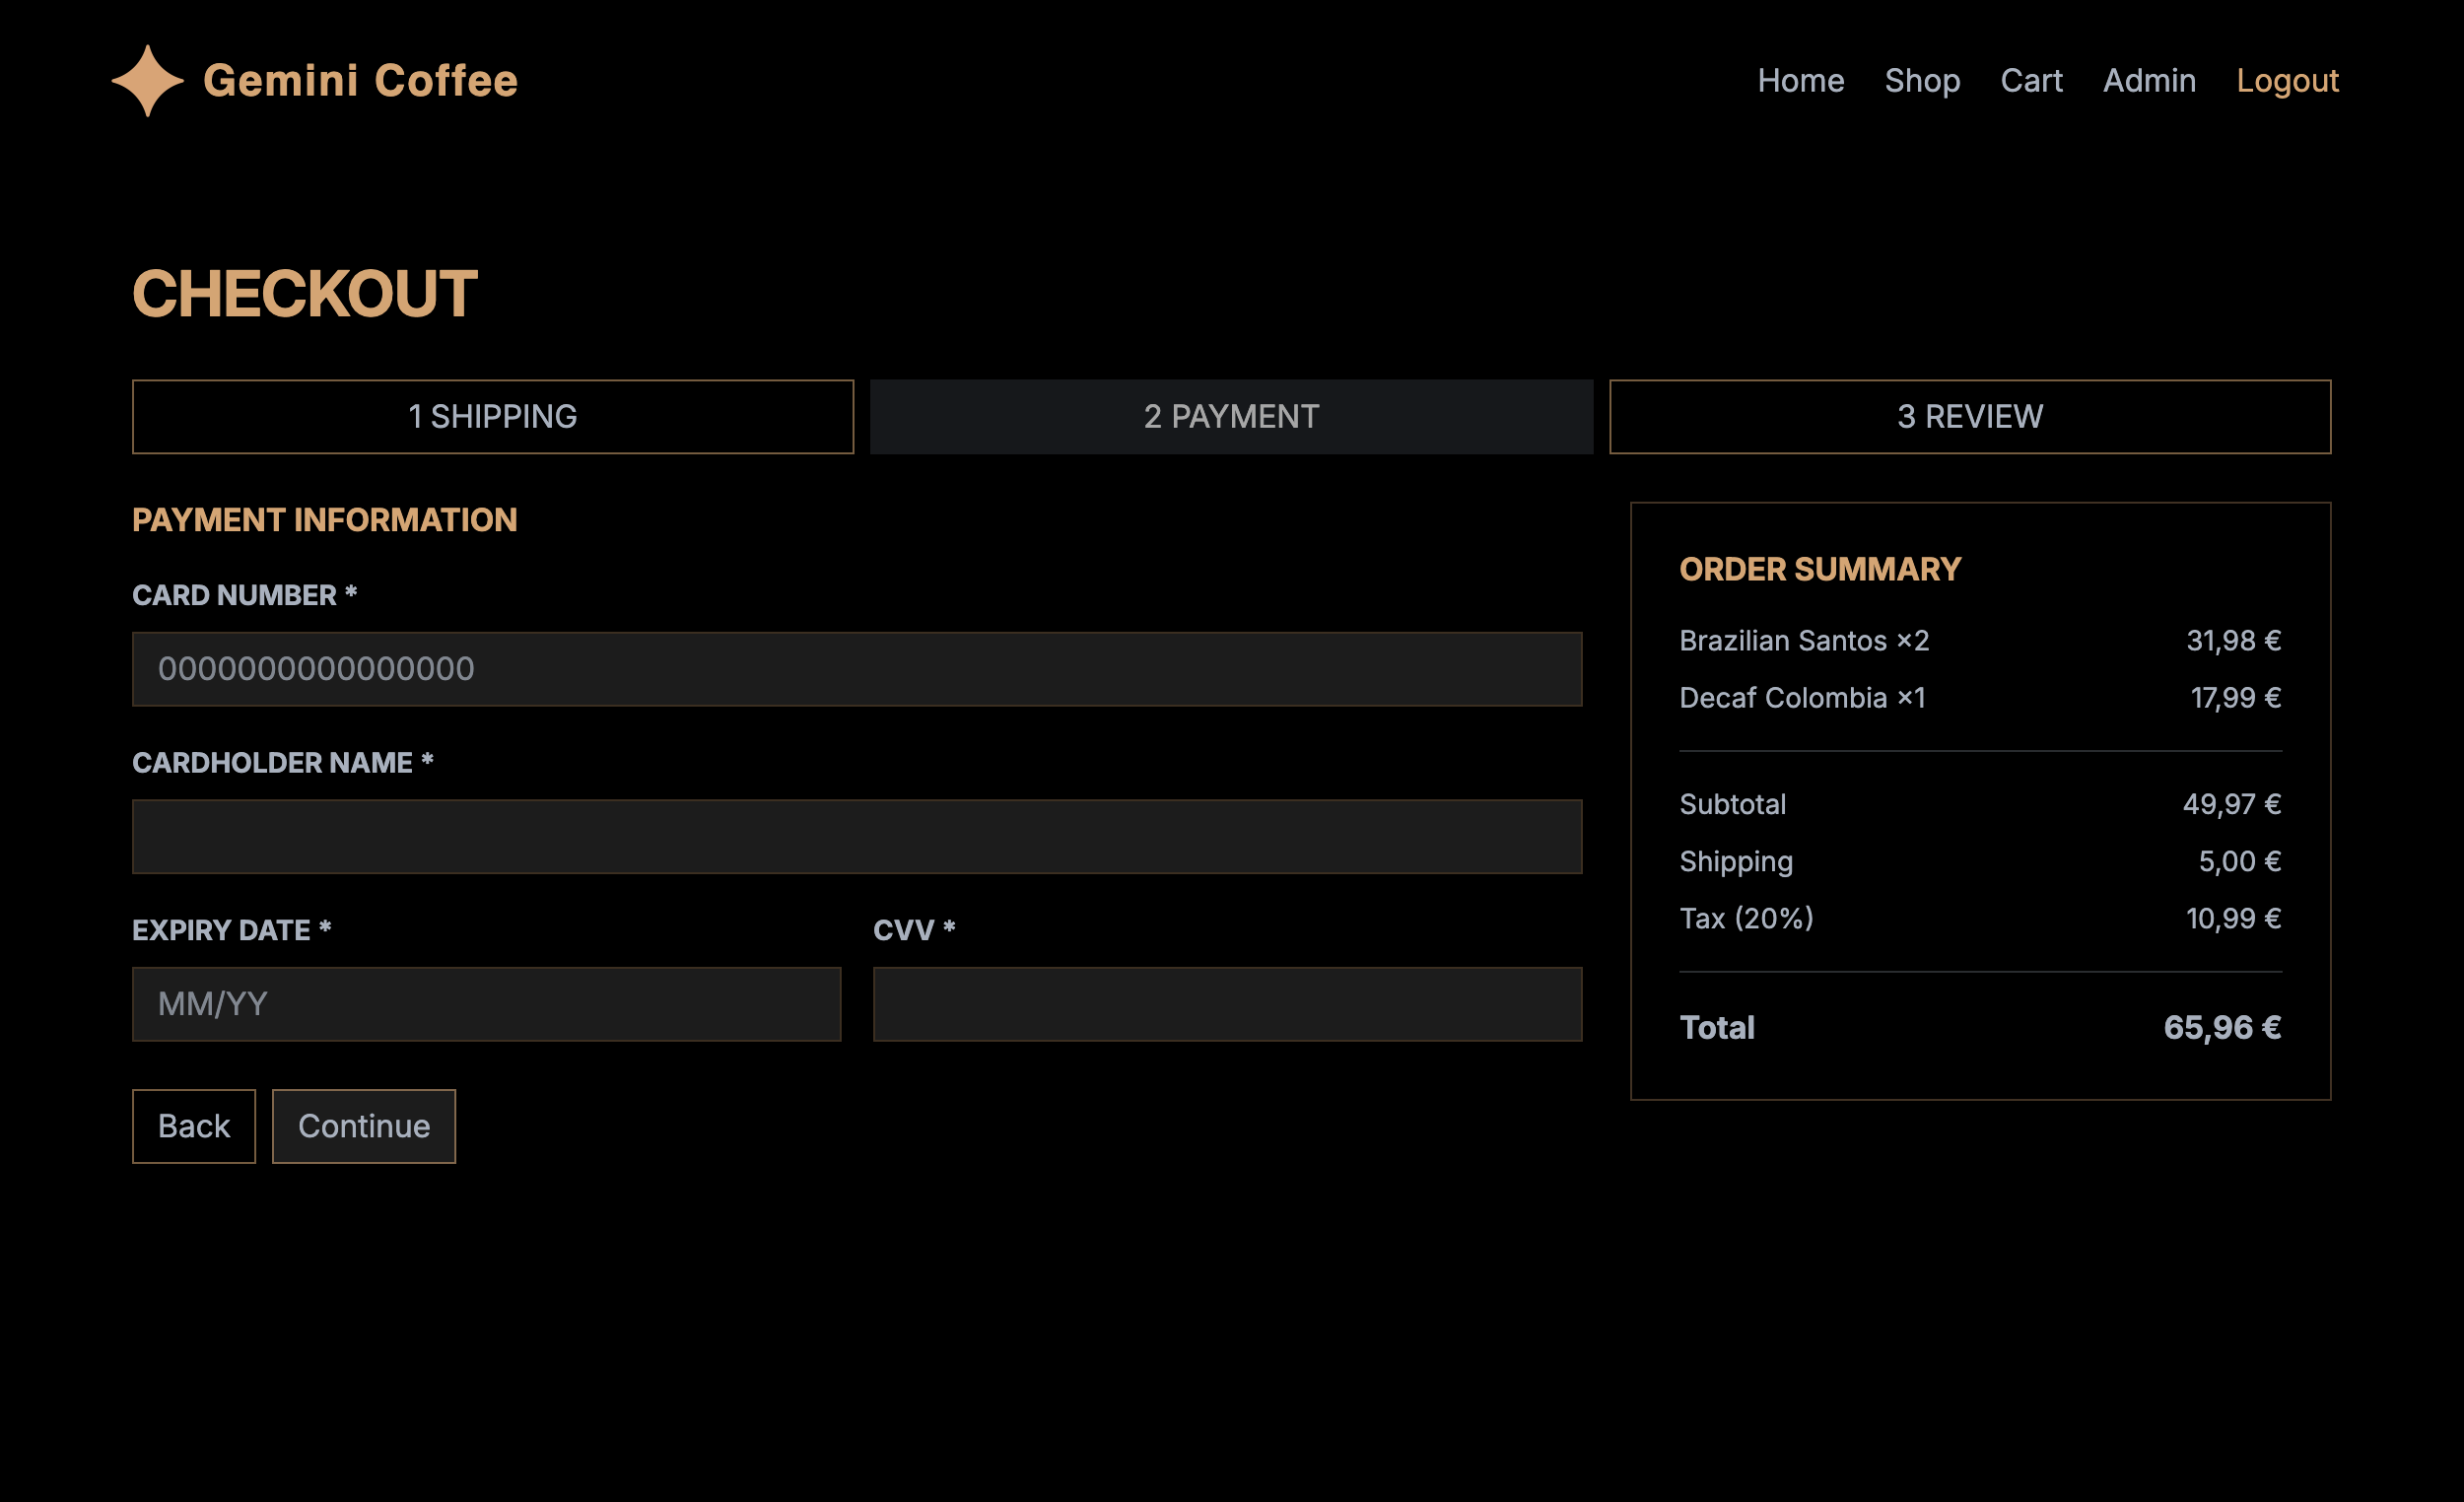
\includegraphics[width=\linewidth, height=0.85\textheight, keepaspectratio]{figures/cart2.png}
  \caption{Krok 1 checkoutu -- výber dopravy a~zadanie doručovacích údajov.}
\end{figure}

\begin{figure}[H]
  \centering
  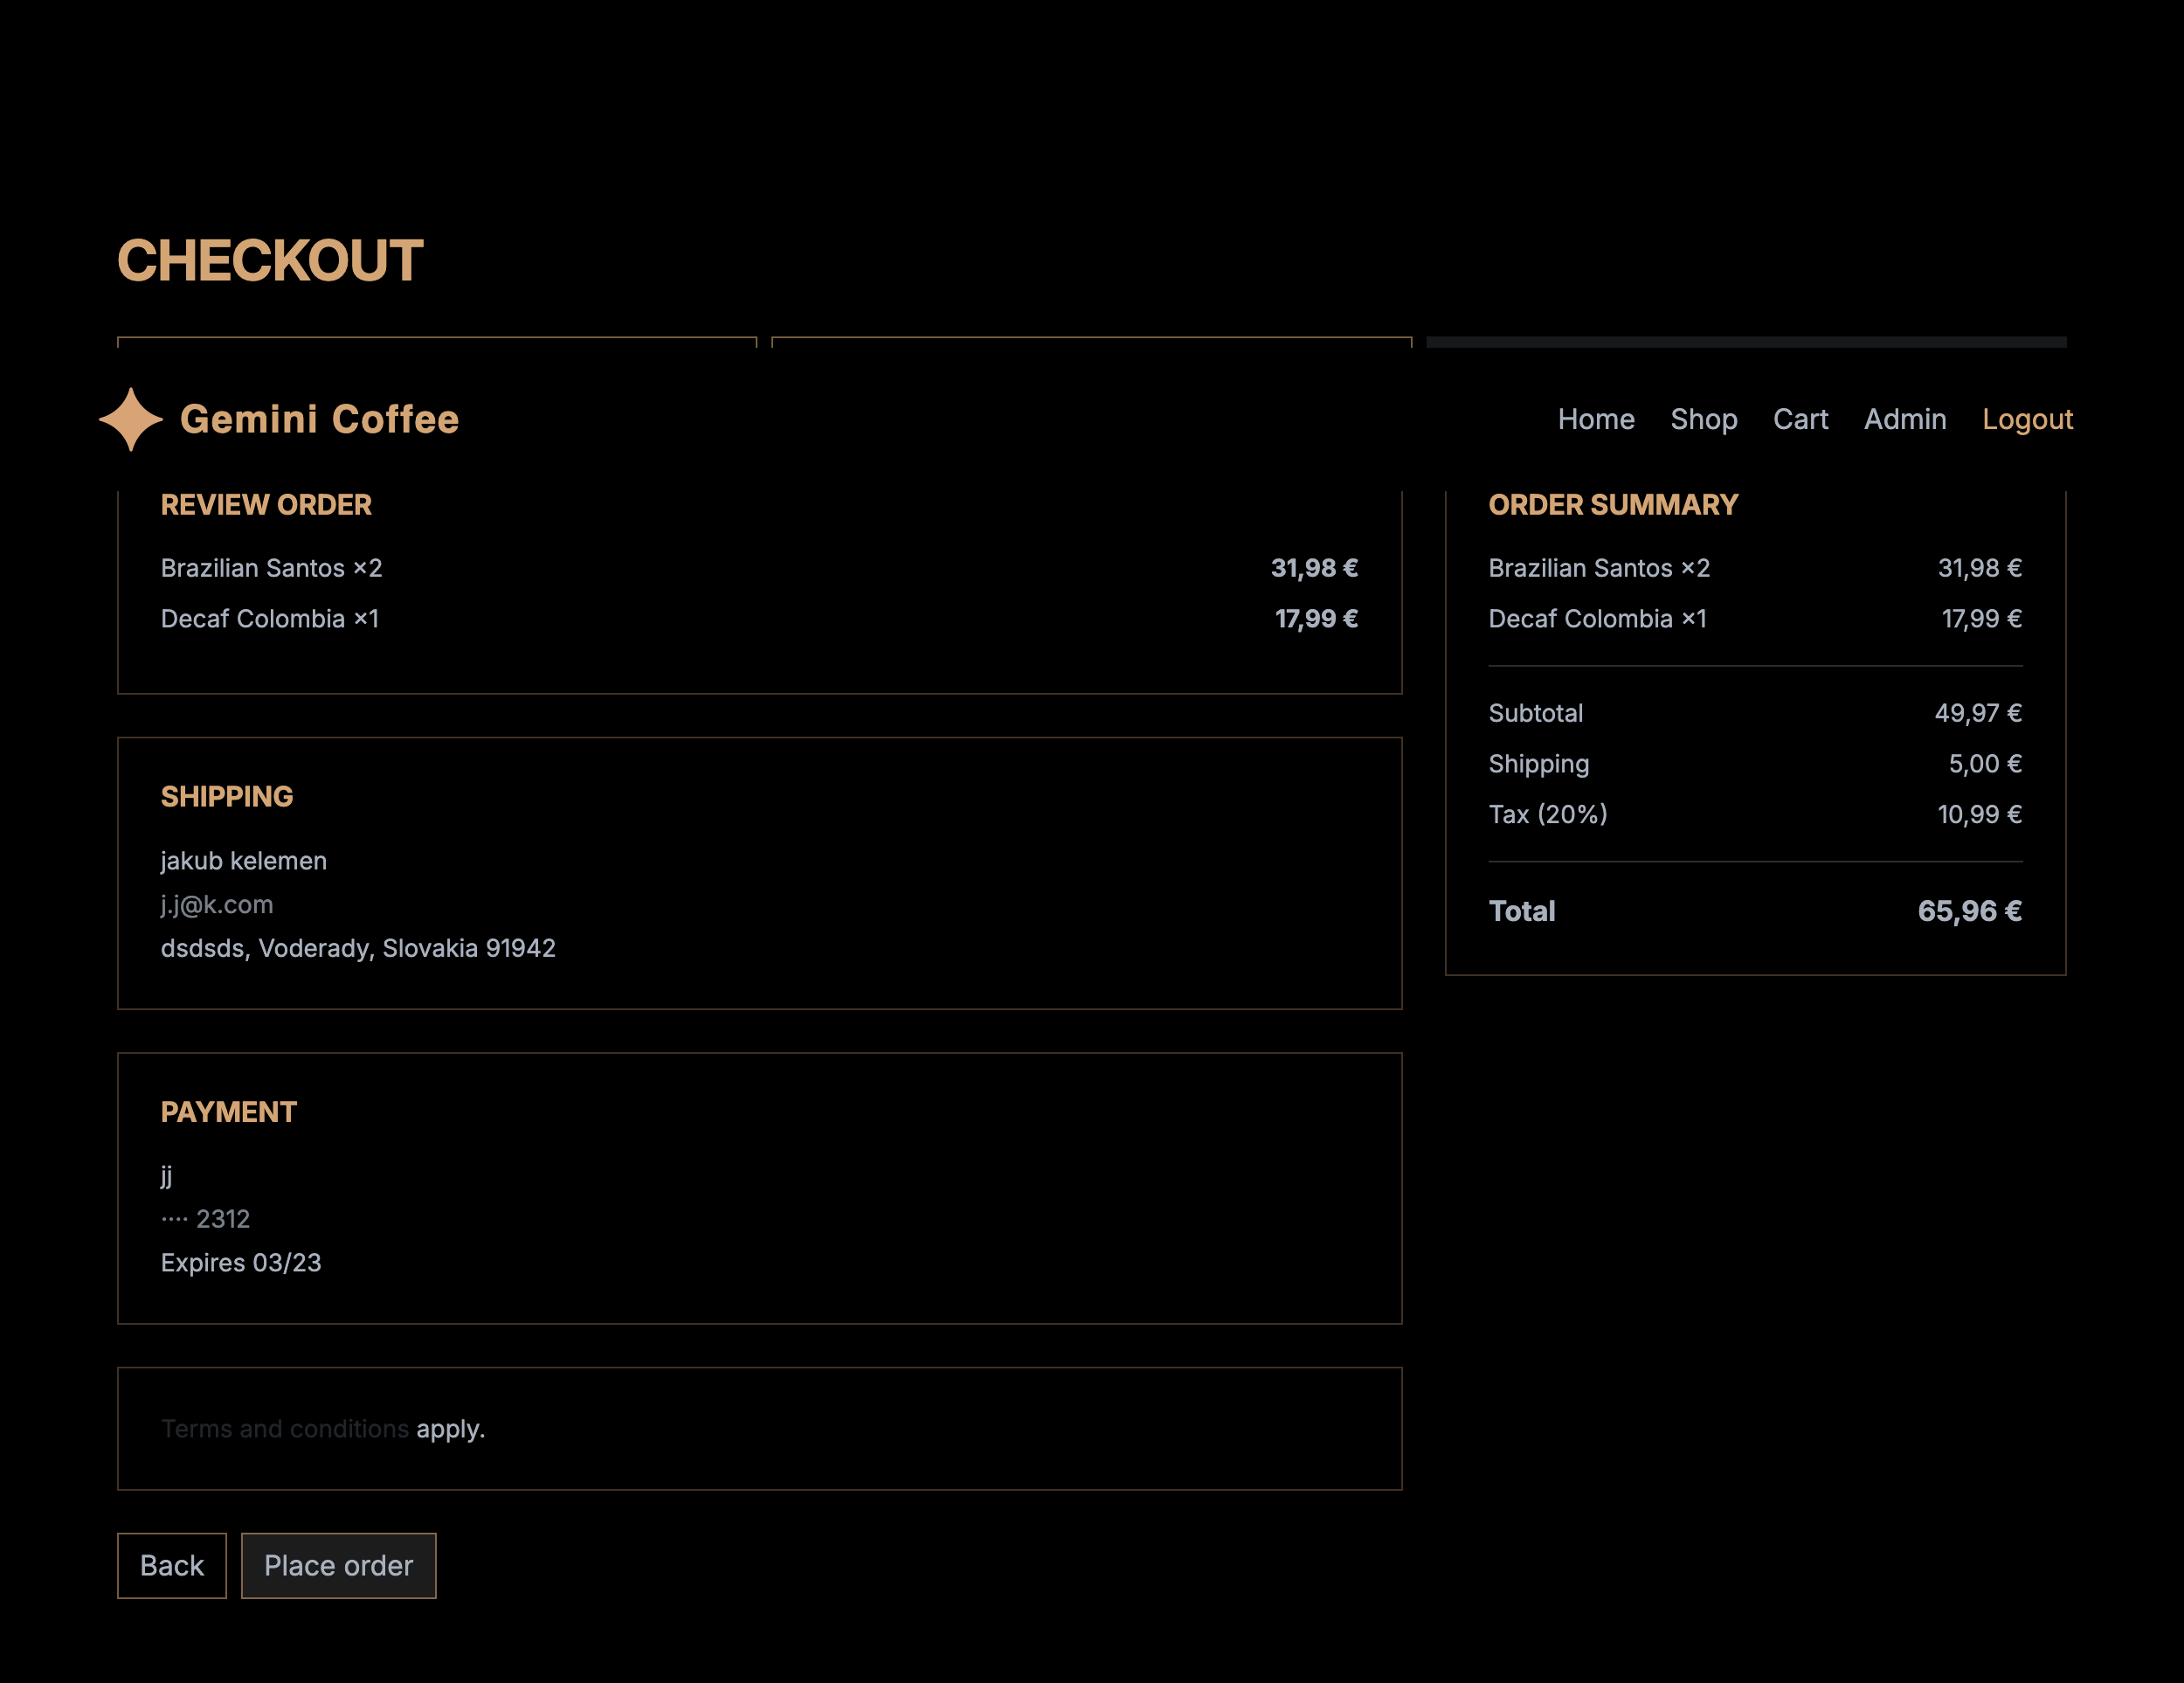
\includegraphics[width=\linewidth, height=0.85\textheight, keepaspectratio]{figures/cart3.png}
  \caption{Krok 2 checkoutu -- zadanie platobných údajov kartou s~validáciou.}
\end{figure}

\begin{figure}[H]
  \centering
  \includegraphics[width=\linewidth, height=0.85\textheight, keepaspectratio]{figures/confirmation.png}
  \caption{Potvrdenie objednávky po úspešnom dokončení checkoutu.}
\end{figure}

\begin{figure}[H]
  \centering
  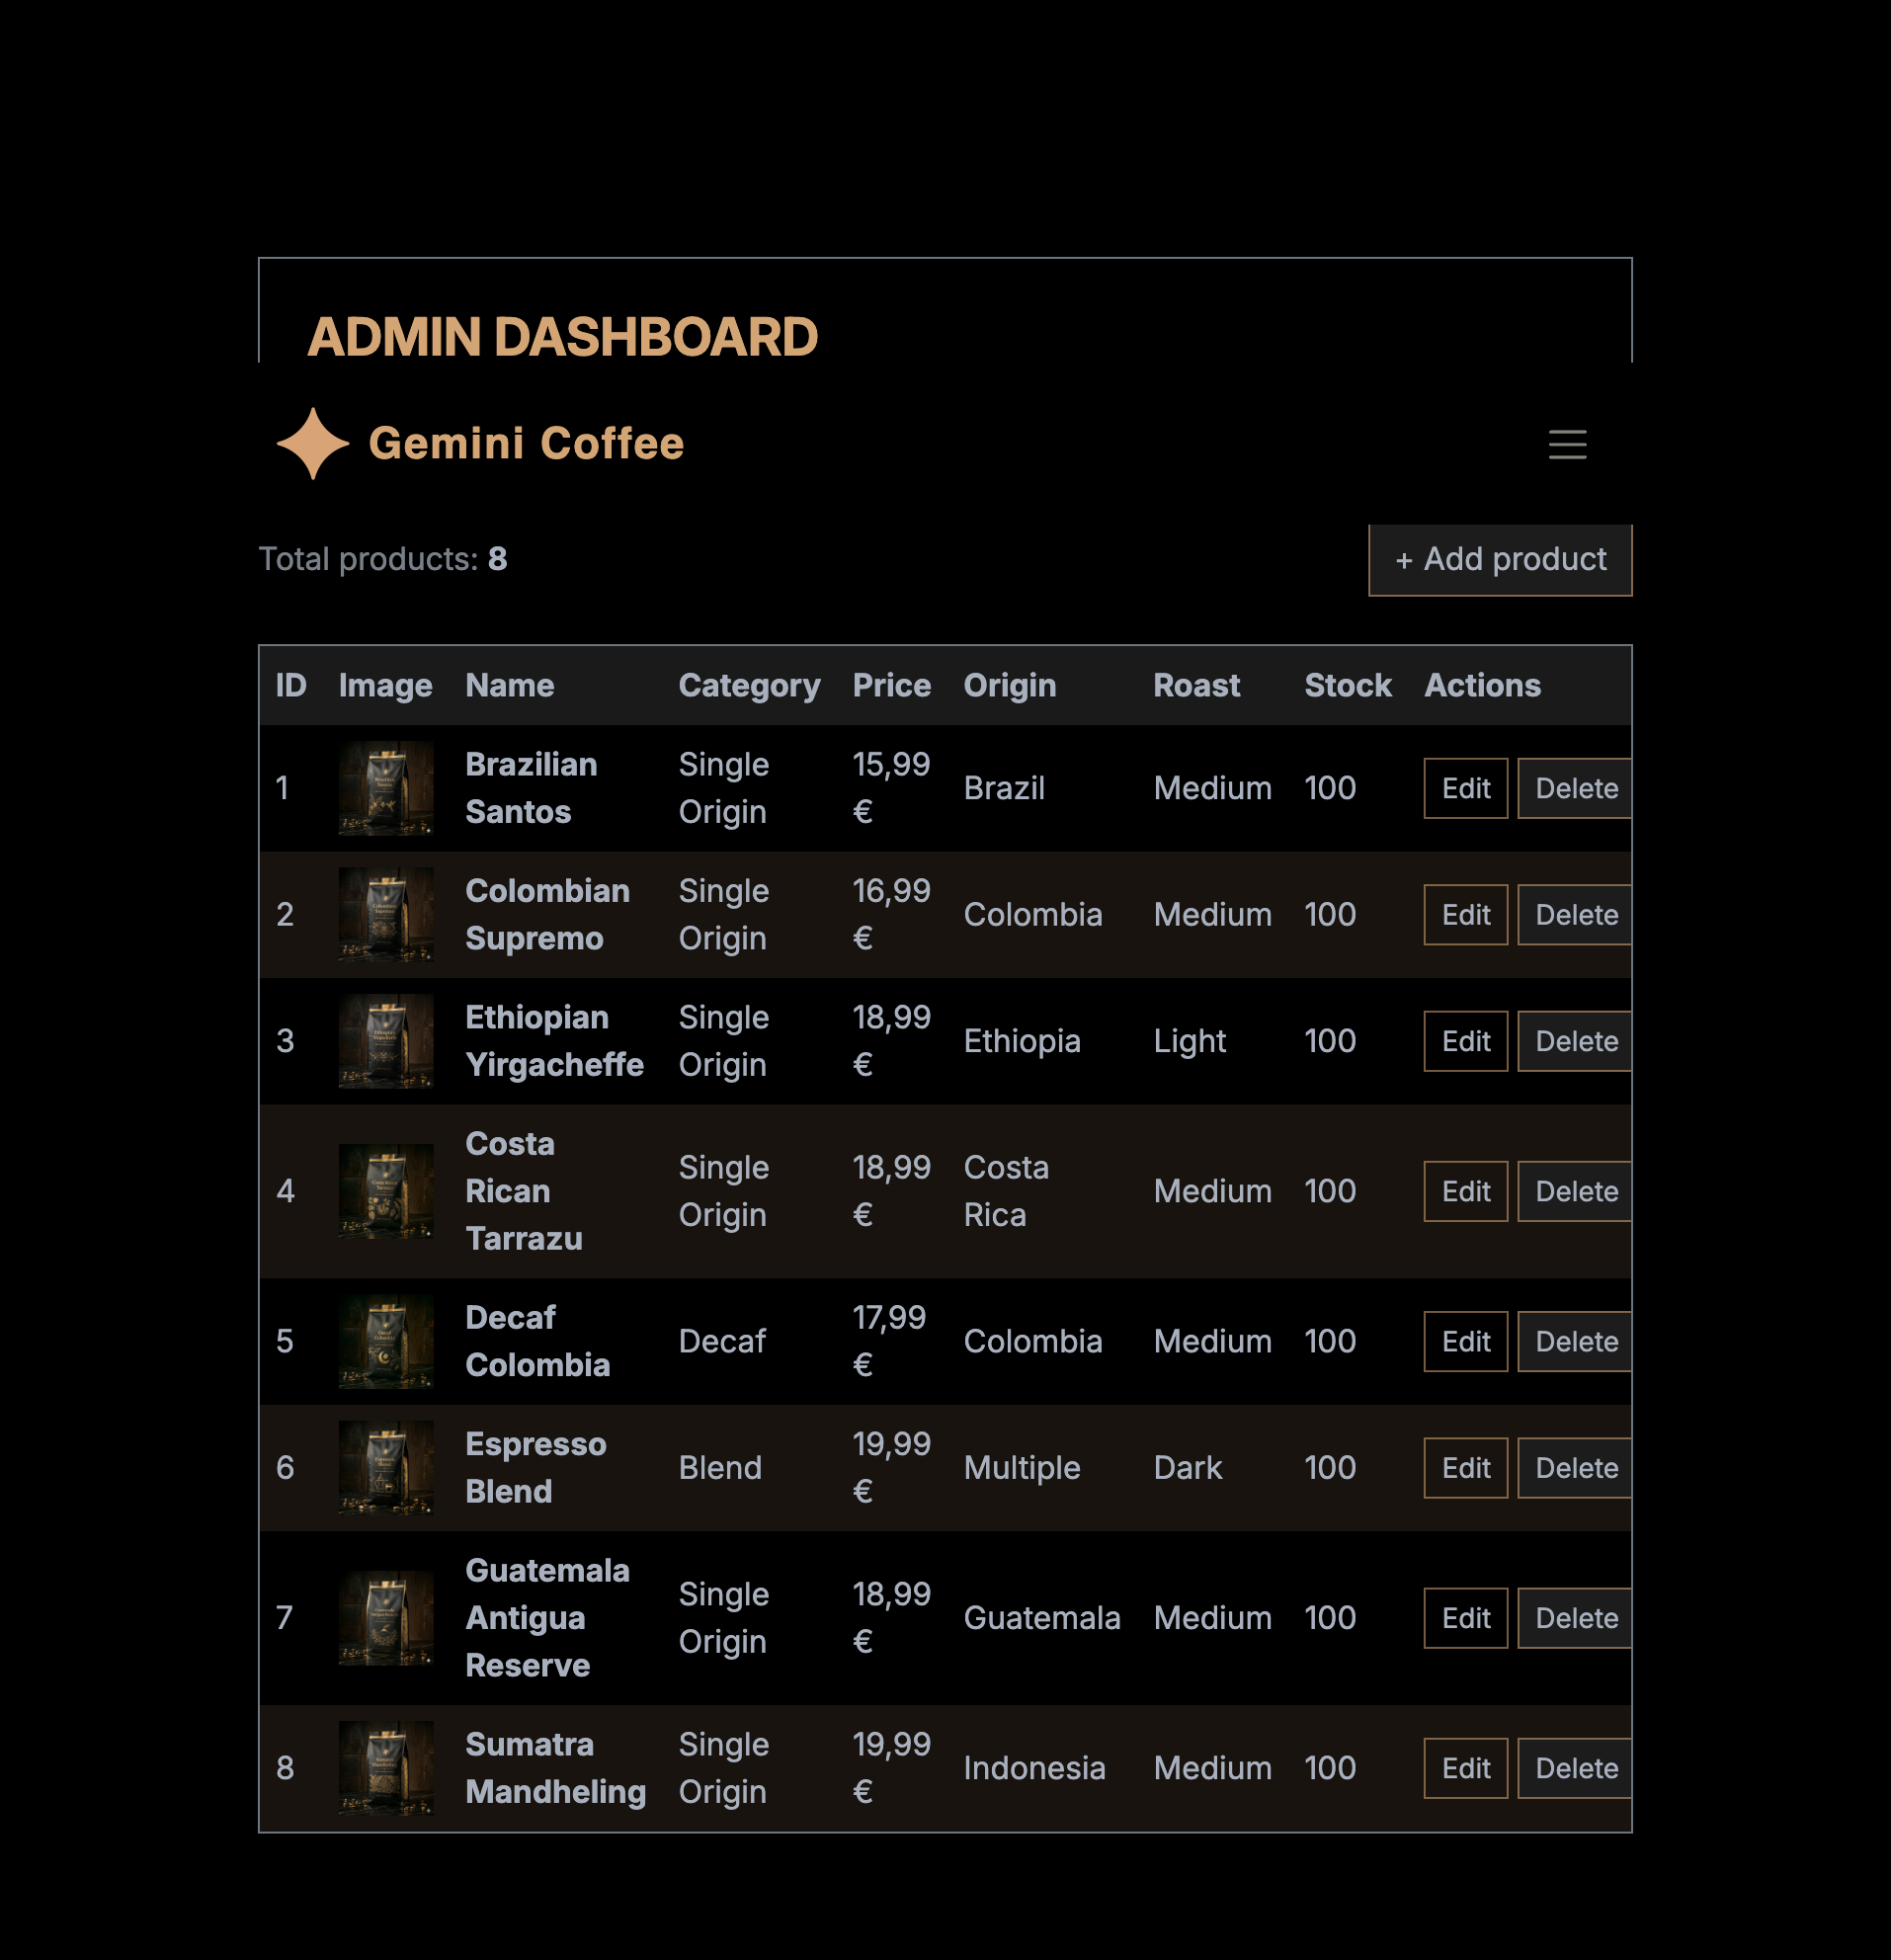
\includegraphics[width=\linewidth, height=0.85\textheight, keepaspectratio]{figures/admin.png}
  \caption{Administrátorský dashboard -- prehľad produktov s~možnosťou editácie a~mazania.}
\end{figure}

\begin{figure}[H]
  \centering
  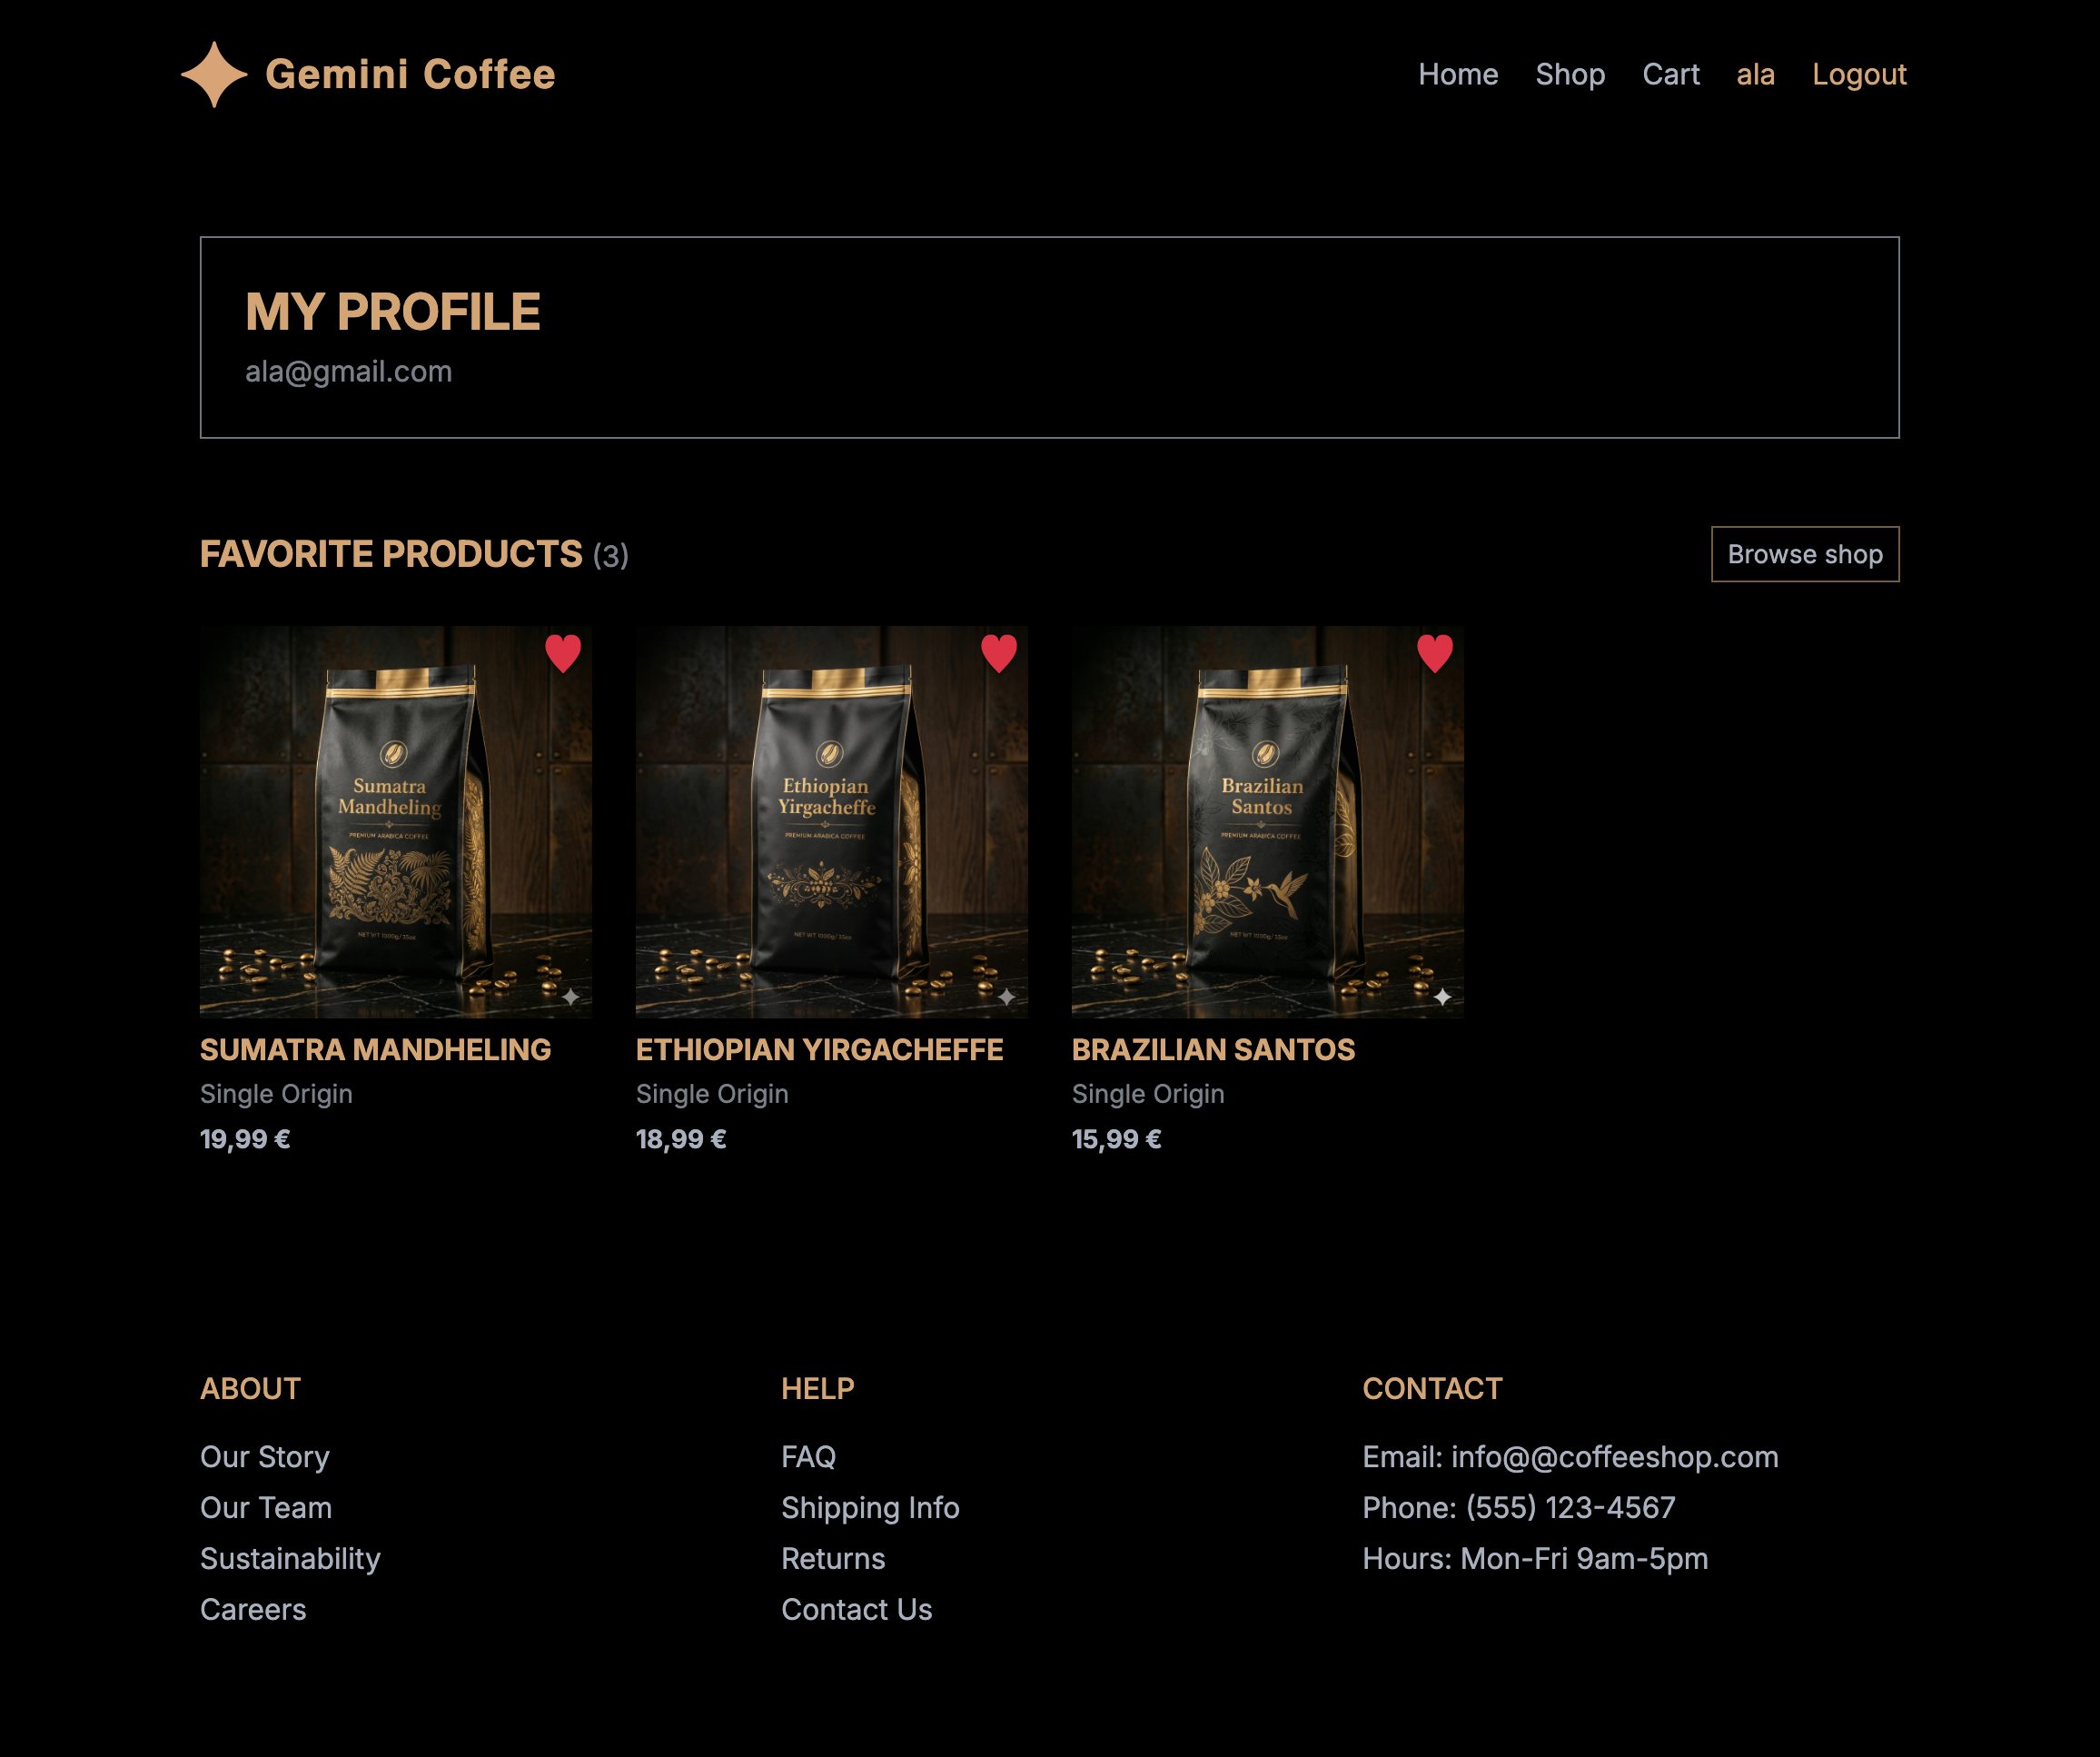
\includegraphics[width=\linewidth, height=0.85\textheight, keepaspectratio]{figures/favourite.png}
  \caption{Profil používateľa s~uloženými obľúbenými produktmi.}
\end{figure}

\begin{figure}[H]
  \centering
  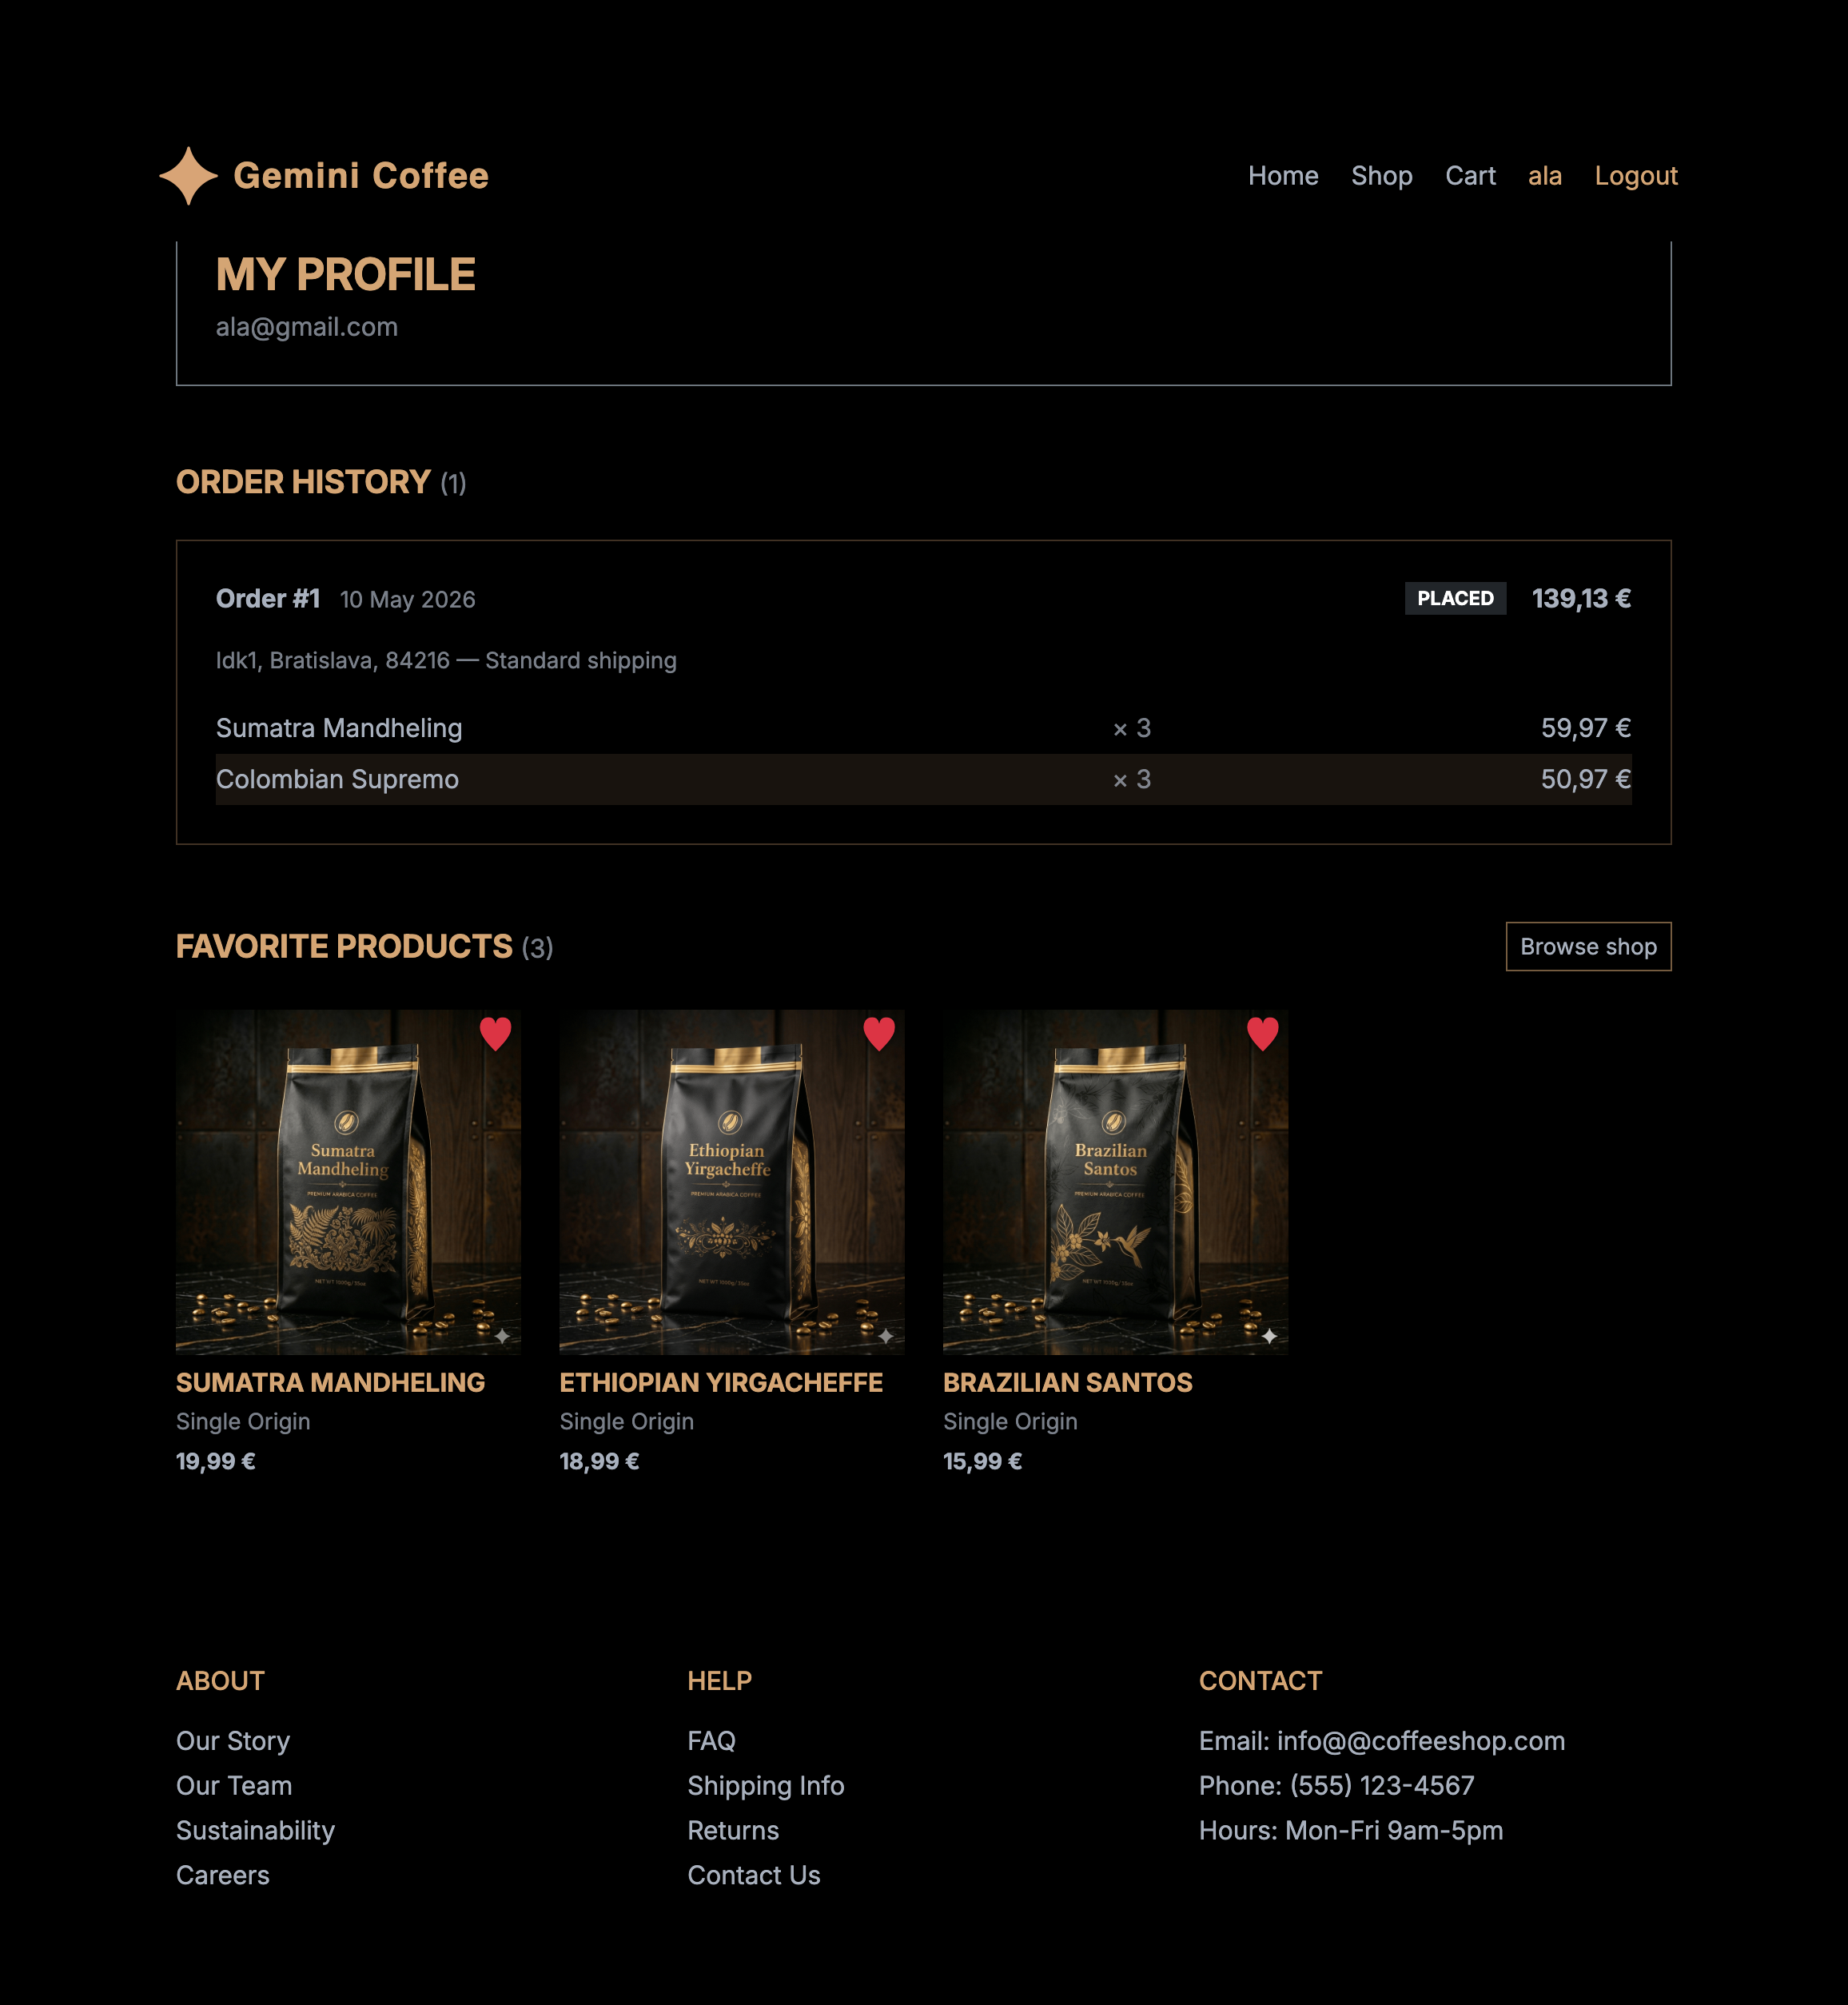
\includegraphics[width=\linewidth, height=0.85\textheight, keepaspectratio]{figures/profile.png}
  \caption{Profil používateľa -- história objednávok s~detailmi položiek a~sekcia obľúbených produktov.}
\end{figure}

\end{document}
